%%%%%%%%%%%%%%%%%%%%%%%%%%%%%%%%%
\chapter{Results with 8 TeV data}
\label{ch:results8}
%%%%%%%%%%%%%%%%%%%%%%%%%%%%%%%%%

%%%%%%%%%%%%%%%%%%%%%%%%%%%%%%%%%
\section{Final $\mWH$ distribution}

\begin{figure}[htbp]
\centering
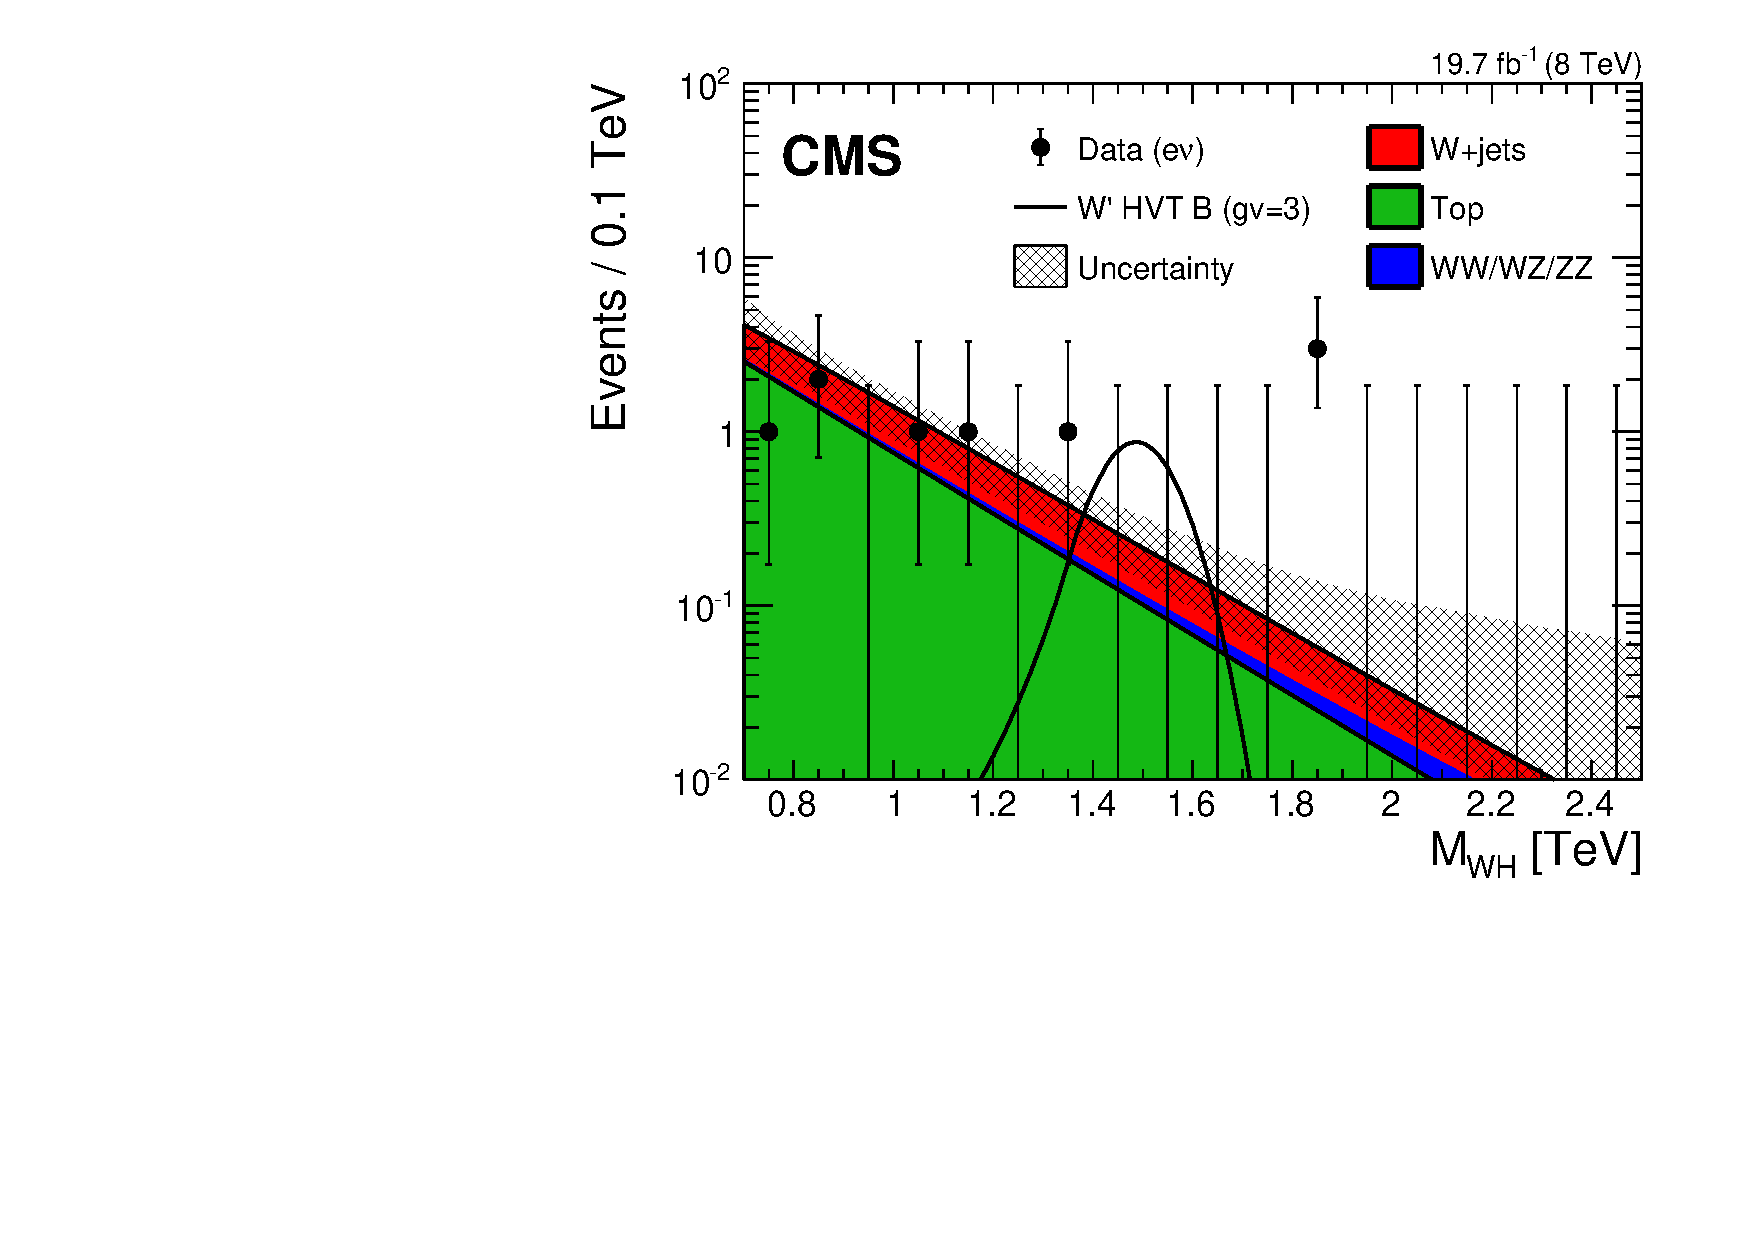
\includegraphics[width=0.49\textwidth]{\cheleven/signal-region-el.pdf}
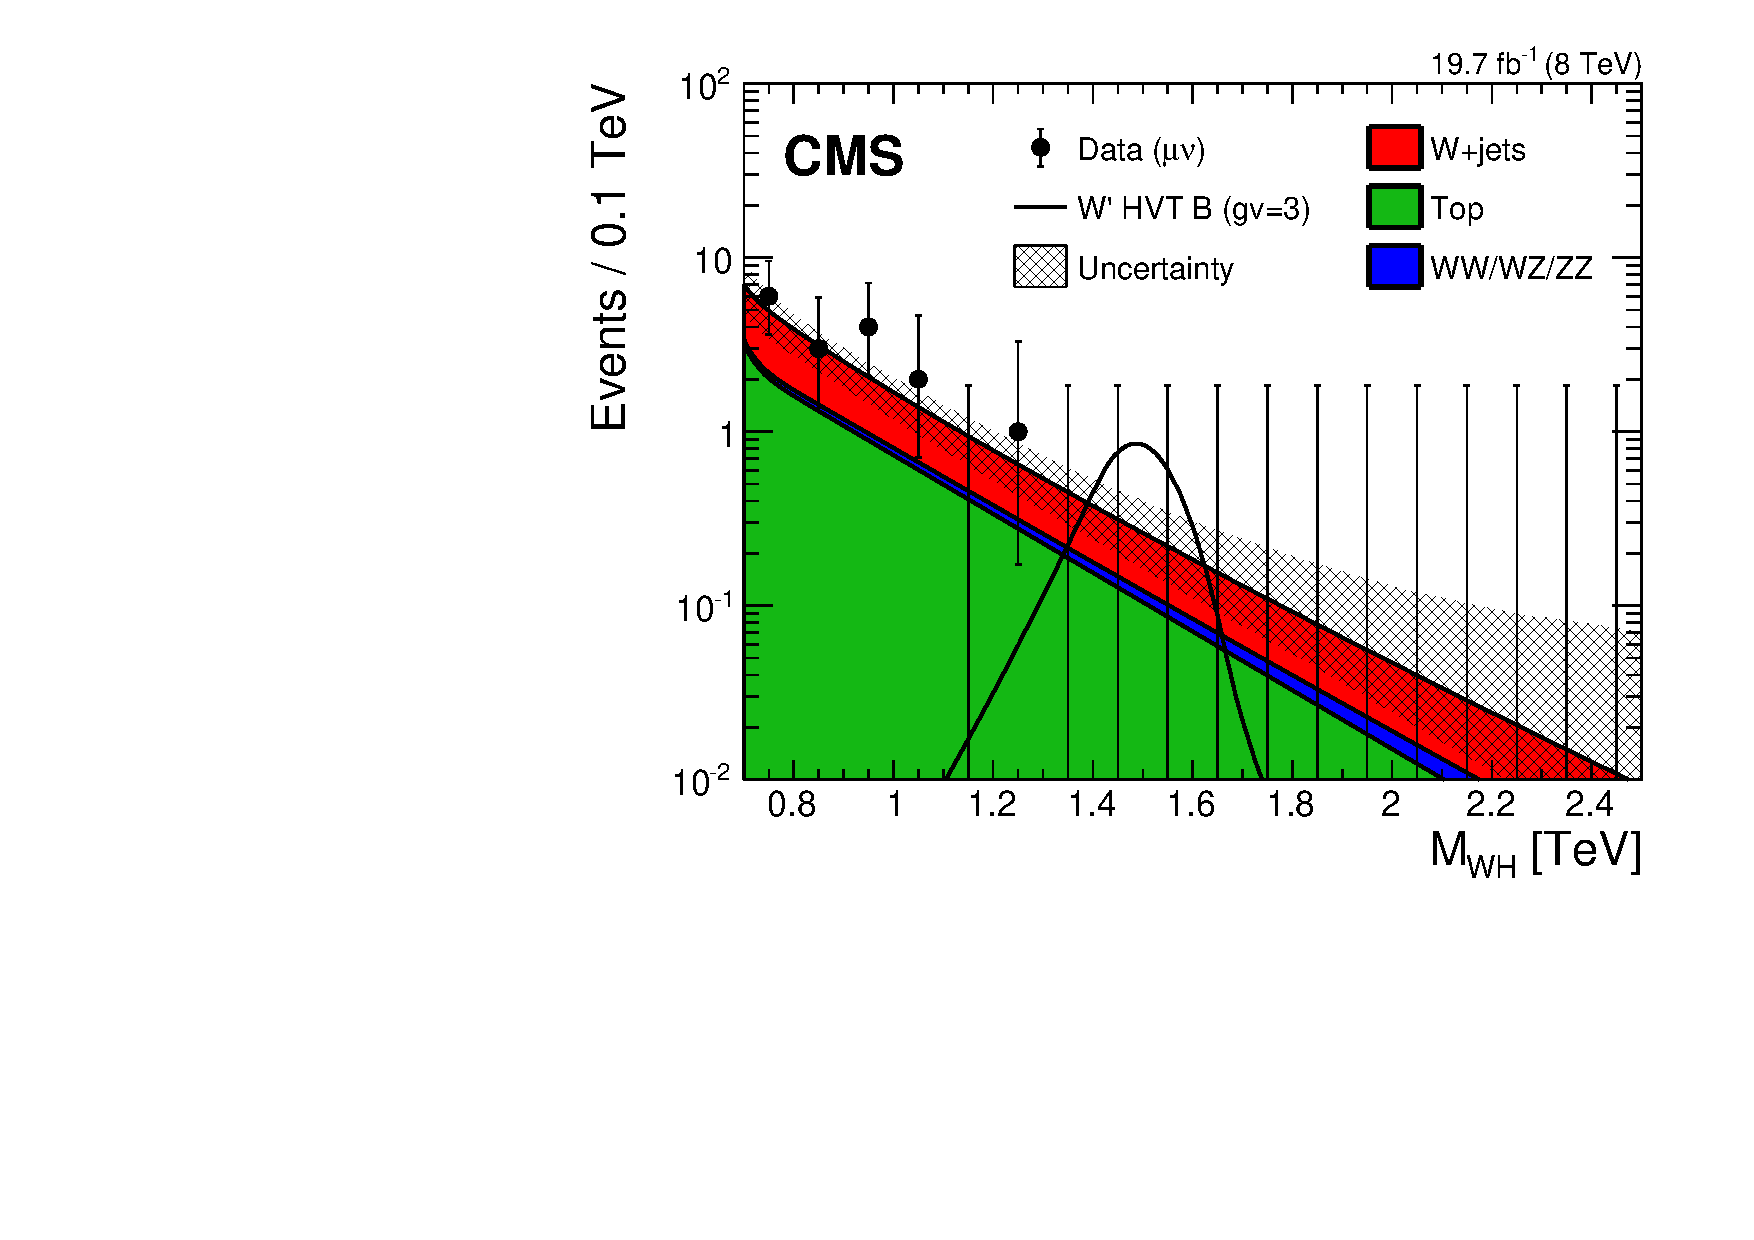
\includegraphics[width=0.49\textwidth]{\cheleven/signal-region-mu.pdf}
\caption{
Final distributions in \mWH for data and expected backgrounds for electron (left) and muon (right) categories.
The 68\% error bars for Poisson event counts are obtained from the Neyman construction~\cite{Garwood}. The hatched region indicates the statistical uncertainty of the fit combined with the systematical uncertainty in the shape. This figure also shows a hypothetical $\PWpr$ signal with mass of 1.5\TeV, normalized to the cross section predicted by the HVT model B with parameter $g_V=3$ as described in Section.
}
\label{fig:MZZwithBackgroundWH}
\end{figure}

%%%%%%%%%%%%%%%%%%%%%%%%%%%%%%%%%
\section{Studies on the excess}

%%%%%%%%%%%%%%%%%%%%%%%%%%%%%%%%%
\section{Significance of the data}

\begin{figure}[htb]
\centering
     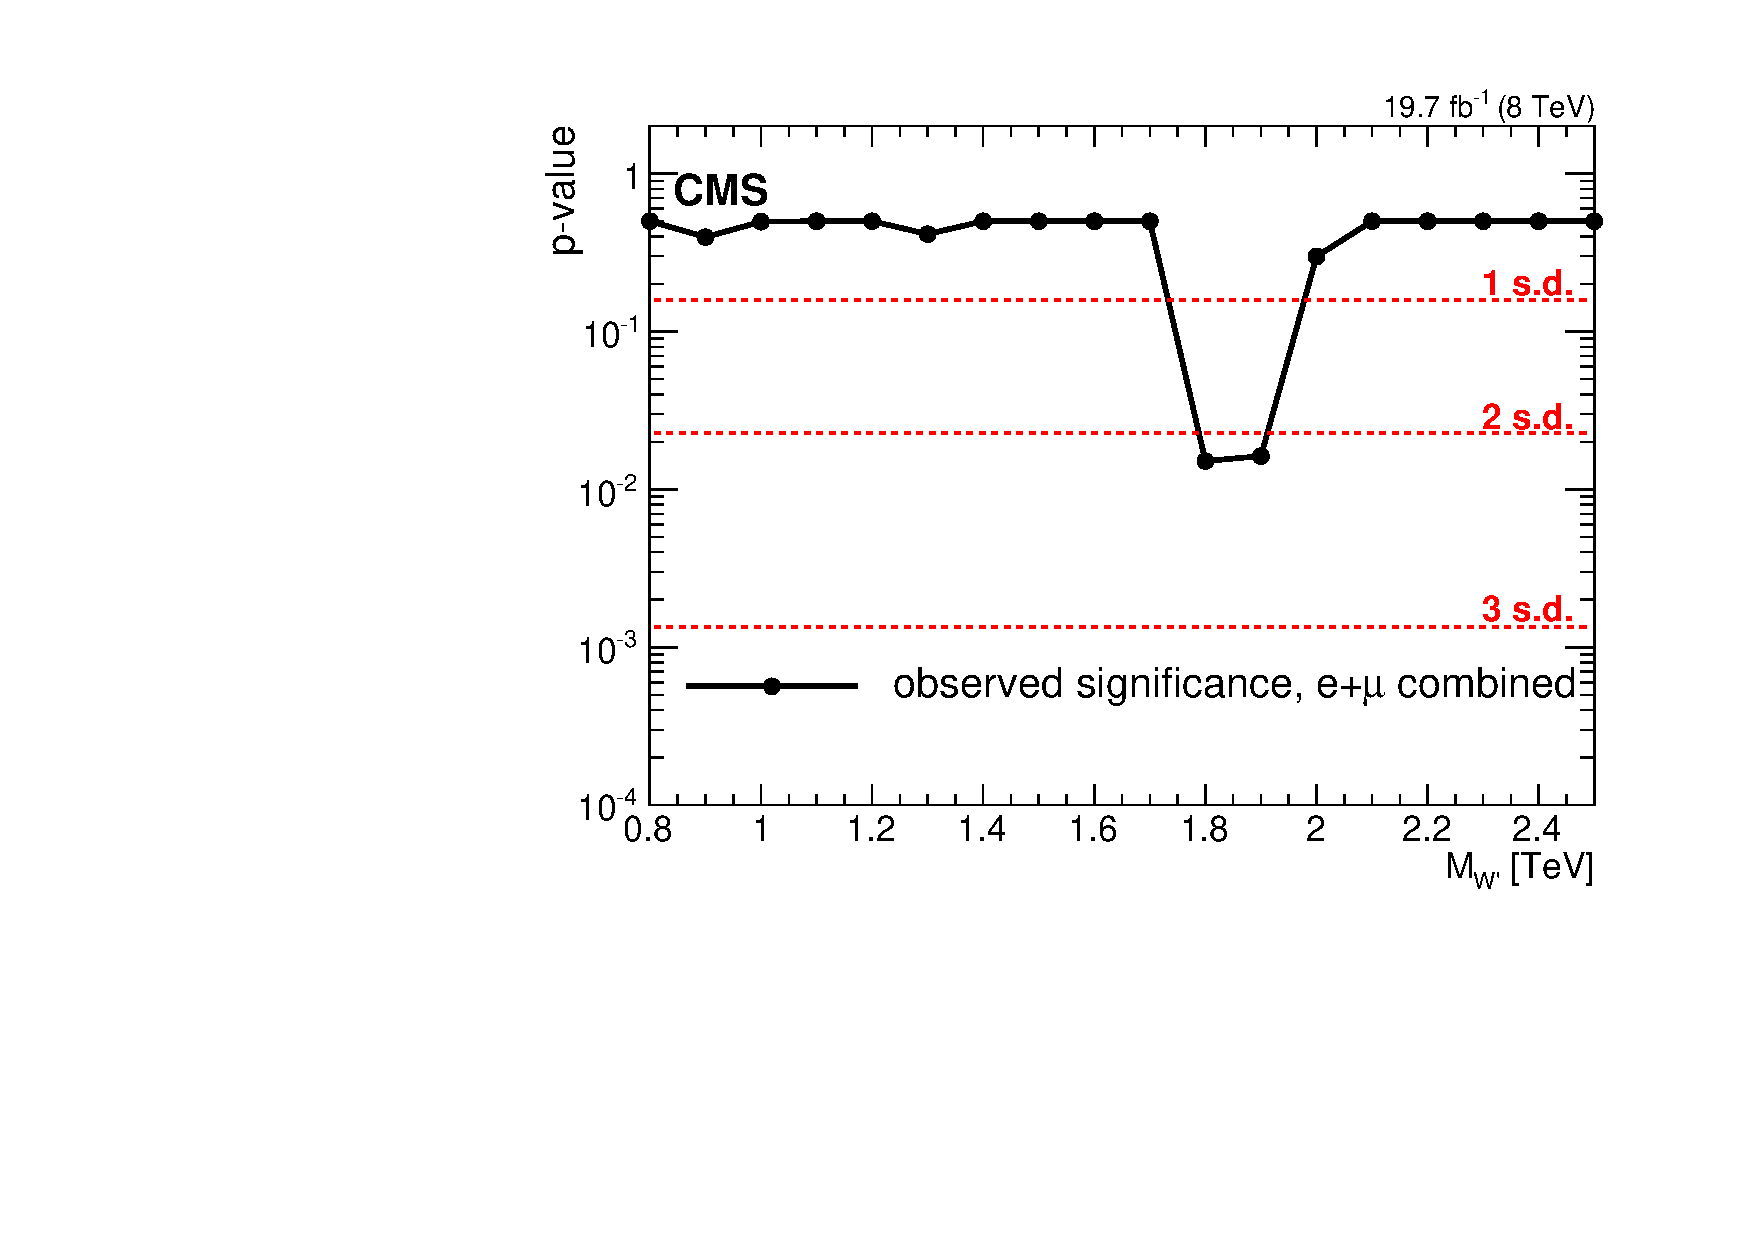
\includegraphics[width=0.49\textwidth]{\cheleven/pvalue_combo.pdf}
\caption{
  Local p-value of the combined electron and muon data as a function of the $\PWpr$ boson mass,
  probing a narrow WH resonance.
}
\label{fig:sig}
\end{figure}

%%%%%%%%%%%%%%%%%%%%%%%%%%%%%%%%%
\section{Cross section limits}

\begin{figure}[htbp]
\centering
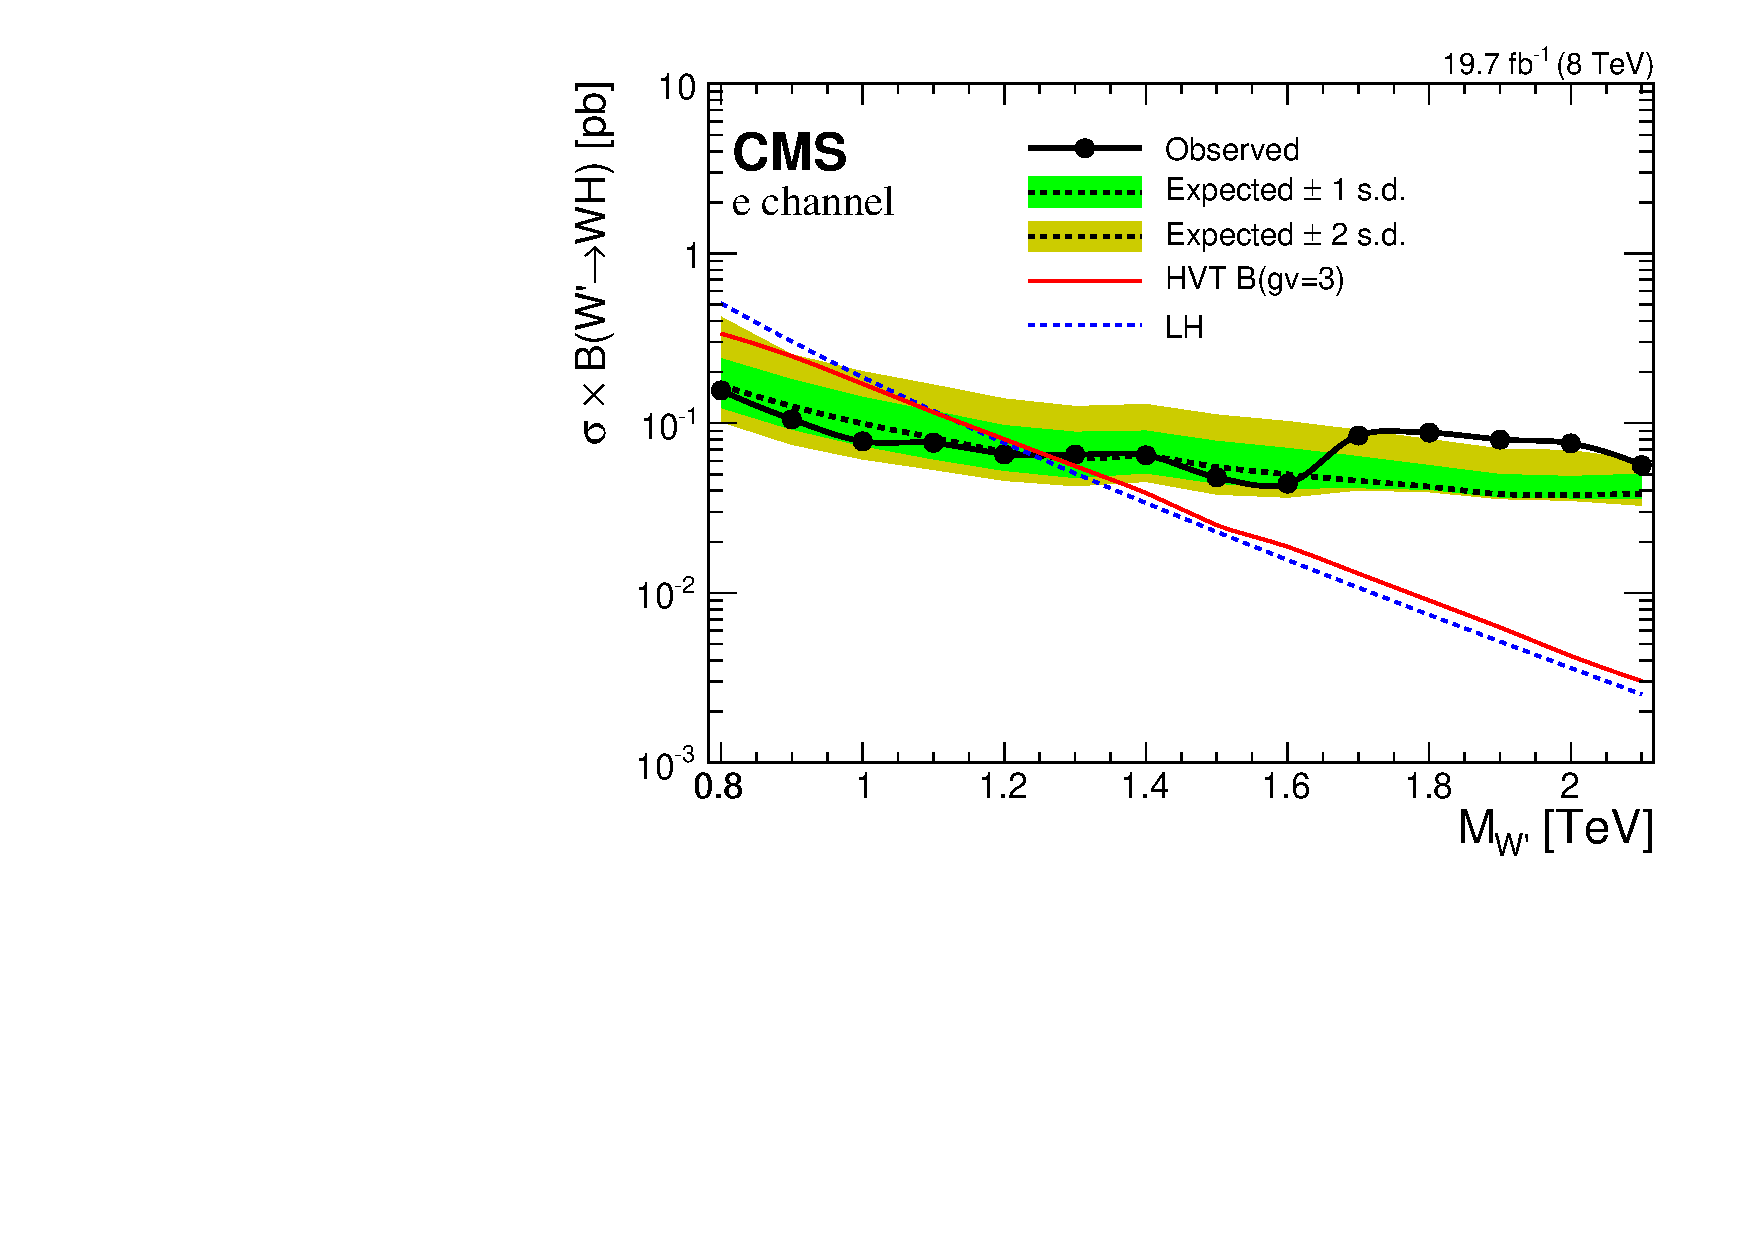
\includegraphics[width=0.49\textwidth]{\cheleven/Lim_el_cls.pdf}
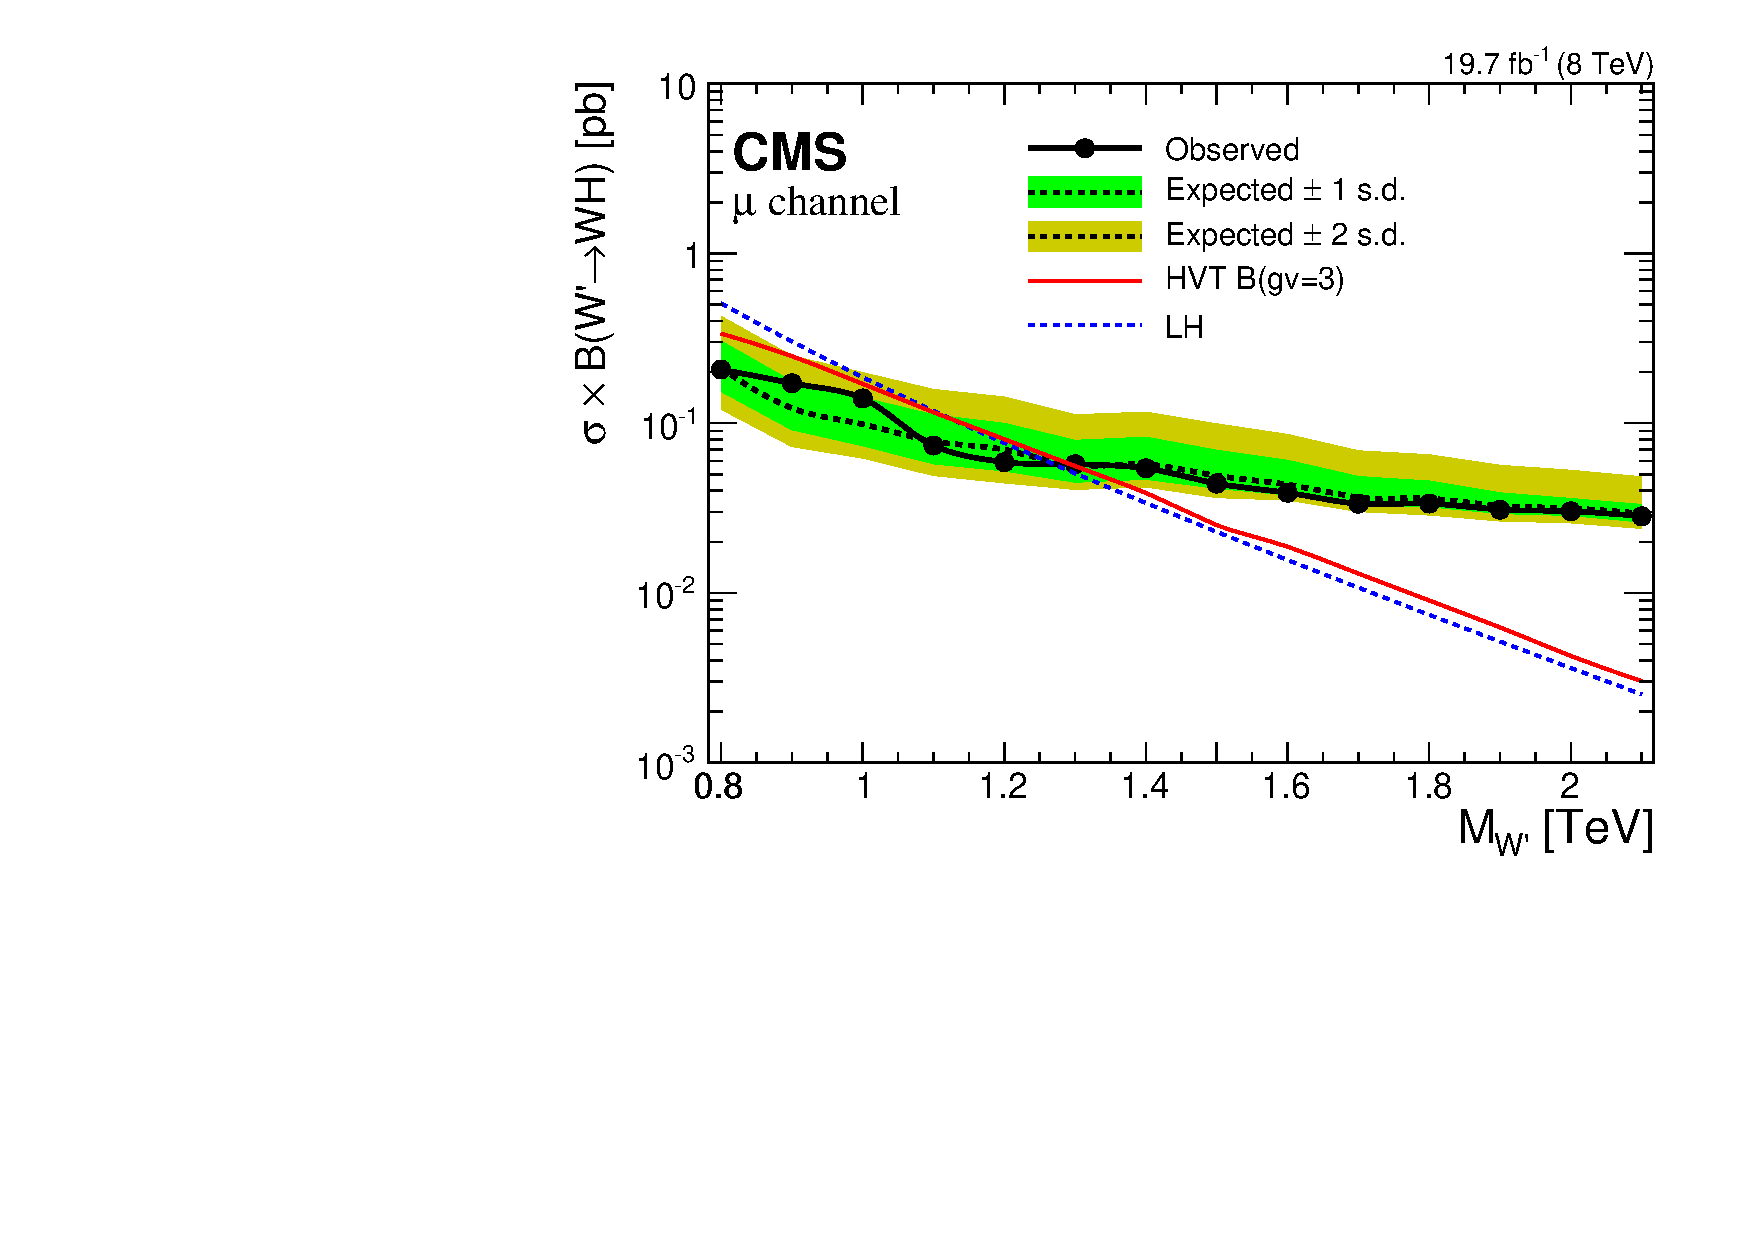
\includegraphics[width=0.49\textwidth]{\cheleven/Lim_mu_cls.pdf}
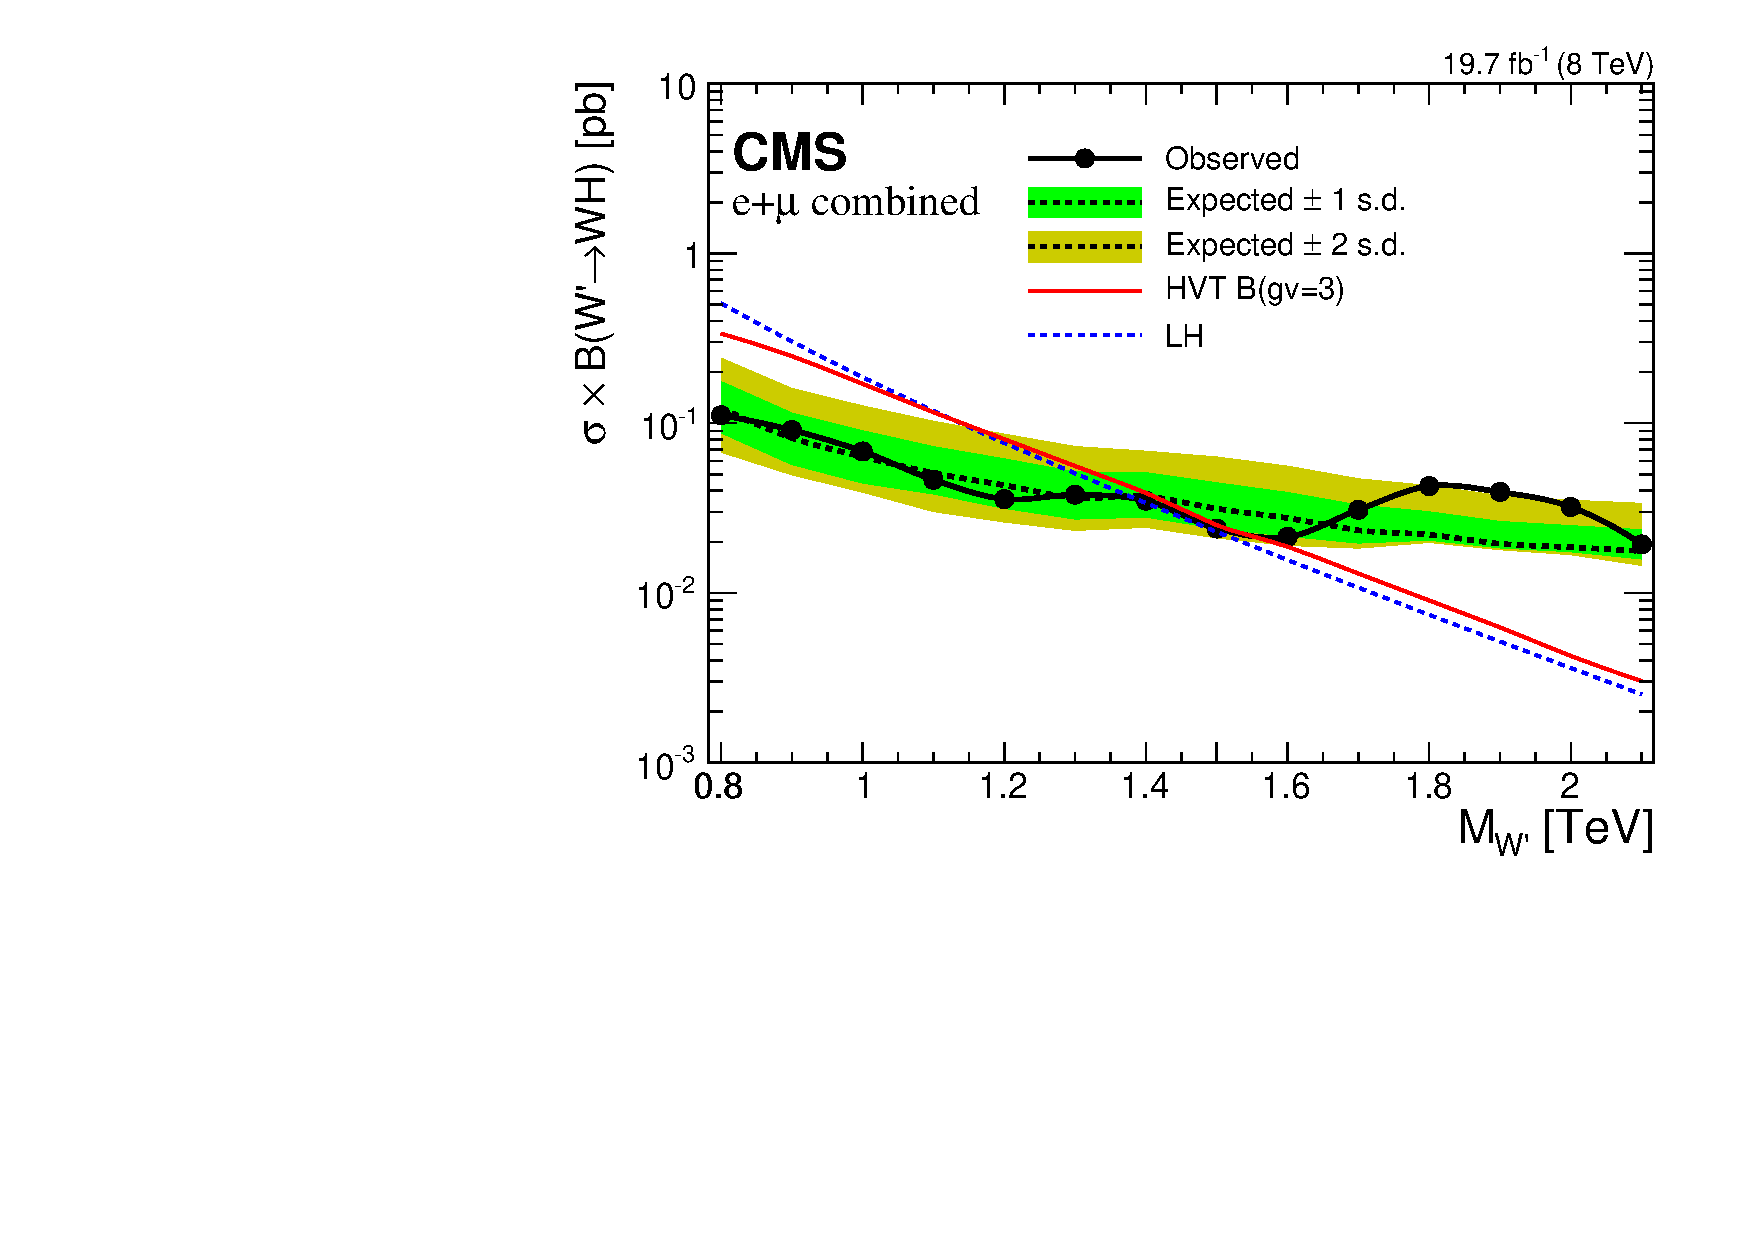
\includegraphics[width=0.49\textwidth]{\cheleven/Lim_combo_cls.pdf}
\caption{
  Observed (solid) and expected (dashed) upper limits at 95\% CL on the
  product of the $\PWpr$ production cross section and the branching
  fraction of $\PWpr\to WH$ for electron (left) and muon (right) channels,
  and the combination of the two channels (lower plot). The products of cross sections and branching fractions for $\PWpr$ production in the LH and HVT models are overlaid.
}
\label{fig:seperateLimits_FullCLs}
\end{figure}